
% Acá entran los puntos 5 y 6
	El algoritmo NLMS se diferencia del LMS en que la correción que se hace es unitaria, es decir que se normaliza la señal de referencia. Así se mejora la convergencia del filtro porque se hace más insensible a los cambios de amplitud de la señal de entrada. La ecuación del filtro NLMS resulta entonces: 

	\begin{equation*}
		w(n) = w(n - 1) + \mu \> \frac{U(n)}{\delta + \|U(n)\|^2} \> [d(n) - U(n)^* w(n - 1)]
	\end{equation*}

	
	En la Figura \ref{fig:ej5} se expone la convergencia de los coeficientes utilizando el algoritmo NLMS, alcanzandose finalmente los valores correctos.
	\begin{figure}[h!]
		\centering
		\includegraphics[width=1.0\textwidth]{graf_ej5.pdf}
		\caption{Convergencia de los coeficientes a partir de la estimación NLMS.}
		\label{fig:ej5}
	\end{figure}

	Se replica el caso de la Sección \ref{sec:ej4} donde se corta el resorte. Al igual que en dicha sección, se impone $k=0,1$ y se ve que cuando $\sigma_N=0,001$ (Figura \ref{fig:ej5_k01}) el algoritmo converge a los valores correctos para todos los coeficientes, mientras que con $\sigma_N=0,01$ (Figura \ref{fig:ej5_k0}) esto no se cumple. 
	
	\begin{figure}[h!]
		\centering
		\includegraphics[width=1.0\textwidth]{graf_ej5_k0.pdf}
		\caption{Convergencia de los coeficientes al cortarse el resorte con $\sigma_N=0,01$.}
		\label{fig:ej5_k0}
	\end{figure}
	
	\begin{figure}[h!]
		\centering
		\includegraphics[width=1.0\textwidth]{graf_ej5_k0bis.pdf}
		\caption{Convergencia de los coeficientes al cortarse el resorte con $\sigma_N=0,001$.}
		\label{fig:ej5_k01}
	\end{figure}

	\pagebreak

	\begin{figure}[h!]
		\centering
		\includegraphics[width=1.0\textwidth]{graf_LMS_vs_NLMS.pdf}
		\caption{Comparación de las convergencias con LMS y NLMS.}
		\label{fig:ej5_comp}
	\end{figure}

	Para comparar los filtros LMS y NLMS se genera la Figura \ref{fig:ej5_comp} que superpone los resultados de ambas estimaciones. Se puede ver que la estimación NLMS converge con una curva más suave que la de LMS mientras que esta última es más ruidosa. La misma conclusión se puede obtener analizando la Figura \ref{fig:ej5_err} que contempla el error entre la estimación y el valor verdadero para las últimas 300 muestras.

	\begin{figure}[h!]
		\centering
		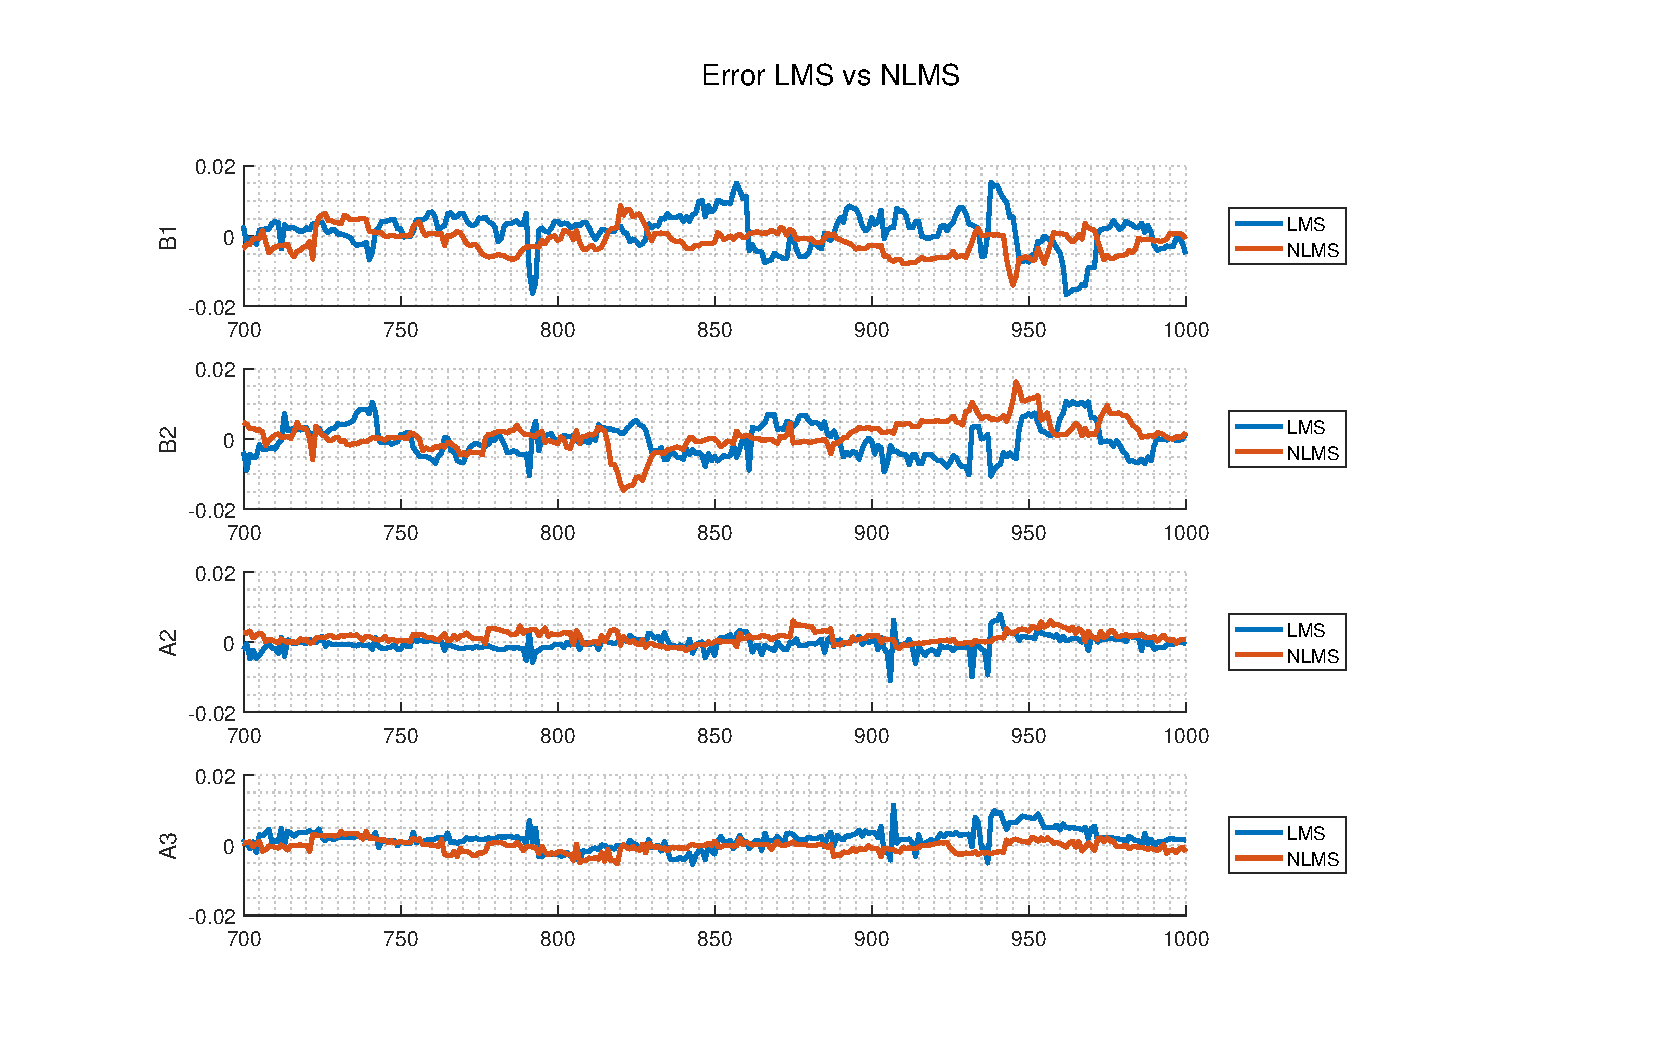
\includegraphics[width=1.0\textwidth]{graf_err_LMS_vs_NLMS.pdf}
		\caption{Comparación de los valores finales de convergencia.}
		\label{fig:ej5_err}
	\end{figure}
	
	En la siguiente tabla, se observa la varianza de los errores de la figura \ref{fig:ej5_err}. Se observa que para NLMS la varianza de los mismos es menor. Se puede concluir, por lo tanto, que las estimaciones en NLMS tienen un error mas suave, y que las del LMS tienen una mayor variabilidad.

	\begin{table}[h!]
		\centering
		\begin{tabular}{ccc}
			\toprule
			$\sigma^2$ & LMS & NLMS\\
			\midrule
			B1 & \num{2.8511e-5} & \num{1.2448e-5} \\
			B2 & \num{2.1332e-5} & \num{1.8342e-5} \\
			A2 & \num{4.3231e-6} & \num{2.6510e-6} \\
			A3 & \num{7.5273e-6} & \num{2.7399e-6} \\
			\bottomrule
		\end{tabular}
	\end{table}

	En cuanto a los resultados de la estimación de los parámetros se obtienen los siguientes resultados para el algoritmo NLMS:
		\begin{table}[h!]
			\centering
			\begin{tabular}{cccc}
				\toprule
				&$m$ (fija)	& $k$	& $b$\\
				\midrule
				Sin corte de resorte&5&$\num{2.9950}$&$\num{2.0008}$\\
				$\sigma_N=\num{.01}$&5&$\num{2.4009}$&$\num{1.9980}$\\
				$\sigma_N=\num{.001}$&5&$\num{0.2236}$&$\num{1.9973}$\\
				\bottomrule
			\end{tabular}
		\end{table}

	Con respecto al sistema funcionando correctamente (sin corte) se ve que el algortimo NLMS estima mejor que el LMS teniendo errores del $0,1$\% versus 1\%. Sin embargo, para el caso del corte de resorte ambos filtros se comportan de manera similar. Ésto puede deberse a que los filtros son en esencia el mismo (salvo la normalización de la corrección) y no pueden lidiar con el problema ante un ruido grande.
